

We now investigate whether word orders as found in natural language optimize the two memory-surprisal tradeoffs.
We compare the memory-surprisal tradeoffs of 52 actual languages to those of counterfactual reorderings.
We cannot just compare to random orderings of individual syntactic trees, as such languages would not have word order regularities.
Therefore, we compare to counterfactual word order grammars.

\begin{figure}
\centering
\begin{dependency}[theme = simple]
   \begin{deptext}[column sep=1em]
	   I \&	   wrote \& risāla \& li \& sadīq  \\
   \end{deptext}
	%   \deproot{3}{ROOT}
   \depedge{1}{2}{obj}
	%   \depedge[edge start x offset=-6pt]{2}{5}{ATT}
   \depedge{1}{4}{obl}
   \depedge{4}{3}{case}
   %\depedge[arc angle=50]{7}{6}{ATT}
\end{dependency}
	\caption{TODO Dependencies example}\label{fig:dependency}
\end{figure}



\subsection{Data}
We draw on corpora annotated with syntactic structures.
The Universal Dependencies project has compiled dependency corpora for several dozen languages~\citep{nivre-universal-2017}.

\paragraph{Dependency Grammar}
In dependency corpora, sentences are annotated with \emph{dependency trees} (Figure~\ref{fig:dependency}).
These are directed trees describing the grammatical relations among words. For example, the arcs labeled ``obj'' represent that the noun in question is the \emph{direct object} if the verb, rather than e.g. the subject or an indirect object.
A dependency arc is drawn from a \emph{head} (e.g. TODO in Figure TODO) to a \emph{dependent} (e.g. TODO).
Dependency trees can be defined in terms of many different syntactic theories \cite{corbett1993heads}.
Although there are some differences in how different formalisms would draw trees for certain sentences, there is broad enough agreement about dependency trees that it has been possible to develop large-scale dependency-annotated corpora of text from dozens of languages \cite{nivre2017universal}.

\paragraph{Corpora}
We considered all languages for which there are Universal Dependencies 2.3 treebanks with a total of at least 500 sentences of training data.
We excluded data from historical languages.\footnote{Ancient Greek, Classical Chinese, Coptic, Gothic, Latin, Old Church Slavonic, Old French.}
This resulted in 54 languages.

For each of these languages, we pooled all available corpora in one dataset.
We excluded corpora that primarily contain code-switched text\footnote{Hindi English corpus}, or text created by non-native speakers.\footnote{ESL, CFL}
Universal Dependencies corpora have a predefined split into \emph{training}, \emph{held-out} (also known as \emph{development}), and \emph{test} partitions.
While larger corpora have all three partitions, smaller corpora often have only some of these partitions.
For most language, we used the predefined data split, separately pooling data from the different partitions. %We did not use the test partitions.
For some languages with little data, there is no predefined training partition, or the training partition is smaller than the other partitions.
In these cases, we redefined the split to obtain more training data:
For these languages, we pooled all the available partitions, used 100 randomly selected sentences as held-out data, and used the remainder as training data.\footnote{This affects Amharic, Armenian, Breton, Buryat, Cantonese, Faroese, Kazakh, Kurmanji, Naija, Thai, and Uyghur.}
For each language, we used the training and held-out sets for estimating the memory-surprisal tradeoff (see Section~\ref{sec:method}).
We provide the sizes of the resulting datasets in Table~\ref{tab:corpora}.



\subsection{Counterfactual Ordering Grammars}
We define ordering grammars, small models of the rules by which languages order syntactic structures into sentences.
Our formalism of ordering grammars adapts the method of \cite{gildea-optimizing-2007, gildea-grammars-2010, gildea-human-2015} to the setting of dependency corpora.

Universal Dependencies defines 37 universal syntactic relations that are used to label dependency arcs across all corpora.
These relations encode cross-linguistically meaningful relations such as subjects, objects, and adjectival modifiers.
We define ordering grammars by assigning a parameter $a_\tau \in [-1,1]$ to every one of these 37 universal syntactic relations.
Relations sometimes have language-specific subtypes; we do not distinguish these subtypes.\mhahn{give an example to make clear what this refers to}

Following Gildea and colleagues, this parameter defines how dependents are ordered relative to their head:
Given a head and a set of dependents, we order each dependents by the parameter $a_\tau$ assigned to the syntactic relation linking it to the head.
Dependents with negative weights are placed to the left of the head; dependents with positive weights are placed to the right.

Ordering grammars describe languages that have consistent word order:
For instance, the subject is consistently ordered before or after the verb, depending on whether the parameter for the verb-subject dependency is positive or negative.

We define baseline grammars by randomly sampling the parameters $a_\tau$.
Such baseline grammars define languages that have consistent word order, but do not exhibit any systematic correlations between the orderings of different dependents.



\paragraph{Discussion}
In actual languages, the ordering of words is largely determined by the syntactic relations (CITE).
However, certain kinds of rules cannot be modeled by our word order grammars, such as rules sensitive to the category of the dependent (e.g., differences between nominal and pronominal objects).
Word order freedom also is not modeled.
In this sense, ordering grammars represent approximations to the kinds of ordering rules found in natural language \cite{gildea-optimizing-2007, gildea-grammars-2010, gildea-human-2015}.



\subsection{Estimating Memory-Surprisal Tradeoff}\label{sec:method}
To estimate mutual informations, we use LSTM recurrent neural networks, the basis of the state of the art in modeling natural language (CITE)\footnote{While Transformers are now better at modeling when large training sets comprising millions of sentences per language are available, they have not reached the level of LSTMs on small/medium training data such as the UD corpora} and predicting the surprisal effect on reading times~\citep{frank-insensitivity-2011, goodkind-predictive-2018}.
%We model language on the level of individual word forms.
We provide data from alternative estimation methods in the SI.


%\paragraph{Data}



%Given a sequence of input words $w_1, ..., w_n \in V$, the model 
%%
%\textbf{TODO I'm describing this in a lot of detail. Alternatively, we can say this is a standard NLP method and refer to the NLP literature for the definition.}
%The first component of such a model is an \emph{embedding matrix} $W_{emb} \in \mathbb{R}^{|V| \times d_{emb}}$, where the \emph{vocabulary} $\mathcal{V}$ is a set, containing the words that occur in the corpus, and $d_{emb} \in \mathbb{N}$ is a fixed parameter.
%This matrix assigns a $d_{emb}$-dimensional vector to each word occurring in the corpus.
%The second component is an LSTM cell $f_{LSTM}$, a nonlinear transformation mapping an \emph{input} vector $x_{i} \in \mathbb{R}^{d_{emb}}$ a \emph{hidden state} $h_i \in \mathbb{R}^{d_{LSTM}}$ and a \emph{cell state} $c_i \in \mathbb{R}^{d_{LSTM}}$ to a new pair of hidden state and cell states $h_{i+1}, c_{i+1} \in \mathbb{R}^{d_{LSTM}}$.
%The LSTM cell $f_{LSTM}$ is parameterized by a matrix of numerical parameters $W_{LSTM}$.
%
%%Such networks estimate the probability of a word in context as follows.
%Given a sequence of input words $w_1, ..., w_n \in V$, the model first retrieves fixed-dimensionality vector representations $x_1, ..., x_n$, where $x_i$ is the row of $W_{emb}$ corresponding to the word $w_i$.
%It then computes a sequence of hidden and cell states by the following recurrent computation:
%\begin{align*}
%	h_1, c_1 &:= 0 \\
%	h_2, c_2 &:= f_{LSTM}(x_1, h_1, c_1) \\
%	\dots \\
%	h_{n+1}, c_{n+1} &:= f_{LSTM}(x_n, h_n, c_n) \\
%\end{align*}
%The vector $h_i$ encodes the result of reading the words $w_1, ..., w_{i-1}$.
%We will write $LSTM(w_1, ..., w_{i-1})$ for $h_i$.
%
%The third component of the recurrent language model is the matrix $W_{output} \in \mathbb{R}^{|V| \times d_{LSTM}}$.
%We obtain per-word predictions of the next word by computing
%\begin{align*}
%	s_i := W_{output} h_i \in \mathbb{R}^{|V|} \\
%	p_i := \operatorname{softmax}(s_i)\in \mathbb{R}^{|V|} 
%\end{align*}
%where the softmax transformation normalizes vectors into probability distributions as follows
%\begin{equation}
%	\operatorname{softmax}(x)_i := \frac{\exp(x_i)}{\sum_{j=1}^{|V|} \exp(x_j)}
%\end{equation}
%Finally, the probability of the word $w_n$ in the context $w_1, ..., w_{n-1}$ is computed as
%\begin{equation}
%	p_\theta(w_n|w_1...w_{n-1}) := \frac{\exp((p_n)_{w_n})}{\sum_{w \in V} \exp(x_w)}
%\end{equation}
%and thus the surprisal is estimated as
%\begin{equation}
%- \log	p_\theta(w_n|w_1...w_{n-1}) := -\log \frac{\exp((p_n)_{w_n})}{\sum_{w \in V} \exp(x_w)}
%\end{equation}
%We discuss the choice of the numerical parameters in the next section.
%

\paragraph{Model and Parameter Estimation}
We use a recurrent neural network with Long-Short-Term Memory cells~\citep{hochreiter-long-1997} (CITE for Neural LM).
This architecture takes as input a sequence $x_1 ... x_N$ of words, and at each time step $t=1, ..., N$, calculates a probability distribution over the next word $w_{t}$ given preceding words $w_1 ... w_{t-1}$: $p(w_t|w_1...w_{t-1})$.

The network is parameterized by a vector $\theta$ of weights determining how the activations of neurons propagate through the network~\citep{hochreiter-long-1997}.
Given a corpus, the numeral parameters of the LSTM are chosen so as to minimize the average surprisal across the training corpus.
%We can think of the LSTM parameters as forming one large vector $\theta$.
At the beginning of training, the parameters $\theta$ are randomly initialized.

The training corpus is chopped into word sequences $w_1 ... w_T$ of length $T$ ($T = 20$ in our experiments).
If $\theta_n$ consists of the LSTM parameters after $n$ training steps, we randomly select a word sequence $w_1 ... w_T$ from the training corpus, and use the LSTM using the current parameter setting $\theta_n$ to compute the per-word surprisals.
We then update the parameter vector:
\begin{equation}\label{eq:train}
	\theta_{n+1} := \theta_n + \alpha \partial_\theta \left(\sum_{i=1}^T \log p_\theta(w_i|w_1...w_{i-1})\right)
\end{equation}
where $\alpha \in \mathbb{R}_+$ is the \emph{learning rate}.
When calculating the parameter update, we use three standard methods of regularization that have been shown to improve neural language modeling: dropout~\citep{srivastava-dropout:-2014}, word dropout, and word noising~\citep{xie2017data}.
In this process, the word sequences are sampled without replacement.
Once all sequences have been processed, we start another pass through the training data.
Before each pass through the training data, the order of sentences of the training data is shuffled, and the corpus is again chopped into sequences of length $T$.

After each pass through the training data, the average surprisal at the current parameter setting $\theta_n$ is evaluated on the held-out partition.
We terminate training once this held-out  surprisal does not improve over the one computed after the previous pass any more.



%\paragraph{Regularization}
%Dropout, Word dropout, Word noising
%Any statistical estimation problem faces the 
%The quality of neural network models is further improved by regularization, improving generalization to the full data distribution.
%In the case of neural networks, the most successful regularization methods typically take the form of random modifications to the input and internal activations when computing the gradients in the training updates~(\ref{eq:train}).
%First, we apply \emph{dropout} both to the input vectors $x_i$ and to the output vectos $h_i$, randomly setting individual elements to zero with rate $p_{embedding} \in [0,1]$.
%Second, we apply \emph{word dropout}, randomly zeroing out entire input vectors $x_i$ at rate $p_{word}$.

\paragraph{Choice of Hyperparameters}

The LSTM model has a set of numerical \emph{hyper-parameters} that need to be specified before parameter estimation, namely the dimensionalities of the embeddings $d_{emb}$, the dimensionality of the hidden states $d_{LSTM}$, and the number of LSTM layers $d_{layer}$, the learning rate $\alpha$, and the regularization parameters (dropout rate $p_{embedding}$, word dropout rate $p_{word}$, word noising rate $p_{noising}$).
We choose these parameters so as to minimize the average surprisal on the held-out partition resulting at the end of parameter estimation.

For each corpus, we used Bayesian optimization using the Expected Improvement acquisition function \citep{snoek-practical-2012} to find a good setting of the hyperparameters.
We optimized the hyperparameters to minimize average surprisal on languages generated from random word order grammars.
This biases the hyperparameters towards modeling counterfactual grammars better, biasing them \emph{against} our hypothesis.

For computational efficiency, neural language models can only process a bounded number of distinct words in a single language.
For each corpus, we limited the number of distinct processed words to the $N=10,000$ most common words in the training corpus, a common choice for neural language models (CITE).
Following (CITE), we represented other words by their part-of-speech tags as annotated in the corpora.
This applied to 37 languages, affecting an average of 11~\% of words in this languages.
We believe that this modeling limitation does not affect our results for the following reasons.
First, this affects the same words in real and counterfactually ordered sentences.
Second, all excluded words are extremely infrequent in the available data, occurring less than 10 times (except for Czech and Russian, the languages for which we have by far the largest datasets).
Many of the excluded words occur only once in the dataset (78 \% on average across the affected languages).
This means that any model would only be able to extract very limited information about these words from the available training data, likely \emph{less} than what is provided by the part-of-speech tag.
Third, traditional N-gram models, which do not have this limitation, provide results in qualitative agreement with the neural network-based estimates (see SI).

%Given a corpus, we estimate a language model by training the LSTM on a training partition to maximize the data likelihood, and stopping training once the data likelihood on a held-out partition drops.
%The hyperparameters (number of hidden units, learning rate, etc.) are chosen so as to maximize the likelihood of the held-out partition.
%This procedure helps prevent overfitting the model to the training data, and ensure that it generalizes to unseen data. 



\paragraph{Estimating the Memory-Surprisal Tradeoff Curve}



The quantity $\operatorname{I}[w_t, w_0 | w_1, ..., w_{t-1}]$ in~(\ref{eq:memory-bound}) is equal to the difference 
\begin{equation}
H[w_t|w_1, ..., w_{t-1}] - H[w_t|w_0, w_1, ..., w_{t-1}]
\end{equation}
For each word in the held-out partition, we compute the difference
\begin{equation}
	-\log P_\theta[w_t | w_0, w_1, ..., w_{t-1}] - P_\theta[w_t | w_1, ..., w_{t-1}]
\end{equation}
and take the average over these.
We cut $T$ off at 20, as this is the length of the sequences processed by the model.

We then used linear interpolation to interpolate the surprisal value for memory values in between these values. (TODO make a figure).
This is justified theoretically (TODO maybe discuss when introducing the theorem).

We estimate the unigram entropy $H[w_0]$ by averaging over all models.

%
%\subsection{Discussion: Alternative Models}
%In view of the NLP literature, the following are the main other options that exist for estimating mutual information and probabilities in sequences:
%
%A traditional model uses n-gram models. A challenge of n-gram models is that they do not express any morphosyntactic generalizations. Furthermore, standard n-gram models do not express any generalizations about pairs of words that are not adjacent -- e.g., encoding a generalization about morphological agreement between two words is hard for such a model to capture if the two words are not always adjacent. Both the small scale of available corpora in many languages and free word order in many languages with rich morphology thus seem to make such models unattractive.
%We evaluate our hypothesis using n-gram models in SI Section X, confirming the conclusions obtained from neural models.
%
%A second option is to construct a statistical grammar, such as PCFG.
%The challenge is to encode statistical morphosyntactic generalizations, and to decide which independence assumptions to put into the model.
%One can either decide on a language-specific basis which generalizations to put in (laborious and might introduce bias), or choose a general model family that is rich enough to learn generalizations.
%The second option will make this a machine learning model that, for our purposes, does not seem to be superior to a recurrent neural network.
%



%\subsection{Data}
%\subsection{Setup}
%The recurrent neural network architecture has a range of adjustable parameters such as the number of neurons.
%For each language, we used Bayesian optimization using the Expected Improvement acquisition function (CITE) \citep{snoek-practical-2012} to find a good setting of the hyperparameters, taking average surprisal on random grammars as the objective.
%This biases the hyperparameters towards favoring counterfactual grammars.

%\subsection{Setup}

For each language, we collected data from the actual orderings and from several random grammars.
We collect multiple samples for the actual orderings to control for variation due to the random initialization of the neural network.
For each of the random grammars, we collect one sample.
Data is collected according to a precision-based stopping criterion described in Section (REF).
%We collected data from the actual and random orderings in proportion one to two.
%The stopping criterion will be described below.

%Due to the randomness both in the sequence of training examples and the random initialization of the network weights, the results of the parameter estimation procedure will vary when run multiple times, especially on smaller datasets.
%Informally, due to the finiteness of the dataset, multiple parameter settings are compatible with the available training data.
%Consequently, memory-surprisal tradeoffs estimated on held-out sets will also show some variation.
%Therefore, we collect multiple samples for the actual orderings to control for variation due to the random initialization of the neural network.


%We chose these thresholds based on preliminary simulations which had suggested that these widths were achievable at acceptable computational cost.

%- at least 30 samples from both baseline and real
%
%- for the language-level tradeoff curve, either the fraction is zero or the bootstrapped CI has width $\leq 0.2$.



%
%(1) is bigram MI always greater in real languages?
%
%(2) is the tradeoff curve always lower than for deterministic simple grammar? for deterministic complex grammars? for stochastic simple/complex grammars?


\subsection{Statistics}

We now describe how we compared memory-surprisal tradeoffs between real and baseline languages.

%For each sample, we estim
%For each language, we viewed surprisal as a function of memory.
%We used linear interpolation to obtain surprisal values for all levels of memory.

We want to test whether languages' surprisal-memory tradeoffs better than those of most baseline languages.
%We view surprisal as a function of memory load, so that the curve is defined on all of $\mathbb{R}_+$.
We compare real and baseline languages by evaluating which languages result in lower surprisal at the same level of memory.
We now describe the statistics we use to quantifying the difference between real and baseline languages.
We do everything in a frequentist framework (null hypothesis testing \& confidence intervals), as we can do exact tests and confidence intervals without parametric assumptions.
Maybe we can explain how the tests \& CIs also have reasonable Bayesian interpretations (for the specific methods used here, rejection of the null should guarantee that the posterior of the null hypothesis is small under a wide range of priors.).

\paragraph{Confidence Interval for Medians}
We use a (nonparametric and nonasymptotic) confidence interval for the median surprisal at 40 evenly spaced points of memory (selected individually for each language), using the binomial PDF. \mhahn{some standard stats reference}
We consider the medians over all runs for the real language, and over all baselines grammars.

% yStudyTradeoff_Bootstrap_Parallel_OnlyWordForms_BoundedVocab_BinomialTest_Single_MedianCI.py


\paragraph{CI for Median Difference}
We create (nonparametric and nonasymptotic) confidence interval for the difference between real and baseline median surprisals at each memory value.
\mhahn{the resulting plots are not very intuitive, might scrap this}

% yStudyTradeoff_Bootstrap_Parallel_OnlyWordForms_BoundedVocab_BinomialTest_Single_MedianDiffCI.py


\paragraph{Pointwise Significance Test}
For each memory value $\mu$, we do a nonparametric and nonasymptotic significance hypothesis test against the null hypothesis that at least half of the baseline grammars have lower surprisal than the actual language (Figure~\ref{fig:nhst-pointwise}).
Formally, let $W_-(\mu)$ be the proportion of baseline languages that have strictly lower surprisal than the real language at memory level $\mu$.
We take the real language to be represented by the \emph{sample median}.
For each level $\mu$ of memory, we consider the null hypothesis that
\begin{equation}
	W_-(\mu) \leq 0.5
\end{equation}
%In reality, we do not observe the curve of the real language exactly, but as noisy samples from our computational estimator.
We use the Binomial Test.

%This statistic also should have a reasonable Bayesian interpretation:
% E.g., if the random samples are unimodal, and we do inference over only the median (location family), 



\begin{figure}
	\begin{center}
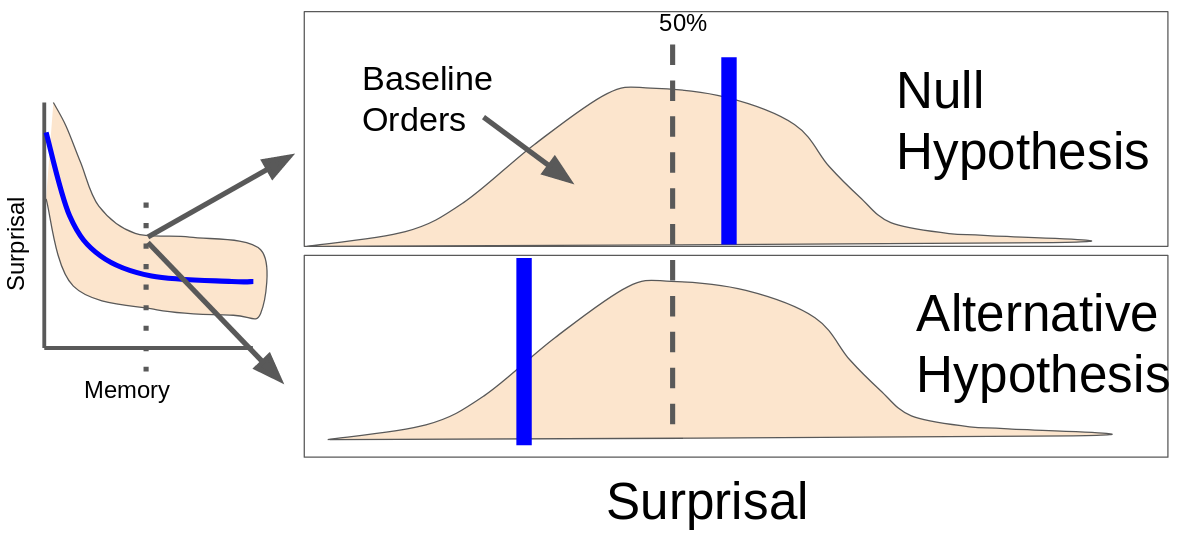
\includegraphics[width=0.45\textwidth]{figures/nhst.png}
\end{center}
	\caption{Illustration for the pointwise null-hypothesis significance test. At a given level of memory, we test against the null hypothesis that at least half of the baseline orders provide lower surprisal than the real language.}\label{fig:nhst-pointwise}
\end{figure}






%For each memory value $\mu$, we do a significance test (nonparametric and nonasymptotic).
%\begin{equation}
%	W_+(\mu) \geq W_-(\mu)
%\end{equation}
%We use the empirical median for the real language.

% yStudyTradeoff_Bootstrap_Parallel_OnlyWordForms_BoundedVocab_BinomialTest_Single.py

%We take the REAL values to be estimated exactly by their medians.



\paragraph{Pointwise Quantile Estimate}
%CI for quantile: % yStudyTradeoff_Bootstrap_Parallel_OnlyWordForms_BoundedVocab_BinomialTest_Single_UnimodalBoundOnQuantile_BothDirections.py
\mhahn{might scrap the CI}

\begin{figure}
	\begin{center}
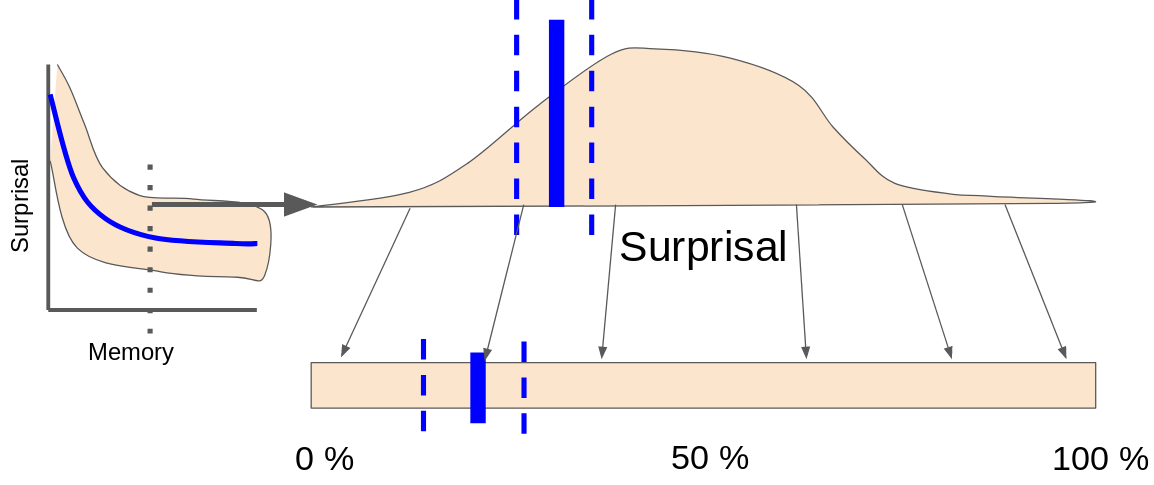
\includegraphics[width=0.45\textwidth]{figures/quantile.png}
\end{center}
	\caption{Illustration for the quantile estimate. At each level of memory, we provide an estimate of the percentage of baseline languages that have lower surprisal than the real language.}\label{fig:quantile-pointwise}
\end{figure}


For each level of memory, we estimate what percentage of baseline languages have lower surprisal than the real language.
This is described in Figure~\ref{fig:quantile-pointwise}.

We derive a CI for the quantile, taking the REAL values to be estimated exactly by their medians.

We want to create a CI at each Memory value for the quantile.

At a fixed memory value $\mu$, let $n_+$ be the better baseline samples, $n_-$ the worse (or equal) ones.

We want to get a confidence bound $q$ on $P_{X \sim Baseline}(X < x_{real})$.

Let $p := P(N_+ \leq n_+ | N_+ + N_-; q)$.
Then output $(0, q)$ as a level $p$ CI for the parameter $P(X < x_{real})$.

We minimize $q$ subject to $p < 0.05$.


This CI is exact in the sense that it does not involve asymptotic approximations or parametric assumptions, but it is extremely conservative.

Also the following does not assume unimodality, and ends up getting about the same intervals
% yStudyTradeoff_Bootstrap_Parallel_OnlyWordForms_BoundedVocab_BinomialTest_Single_UnimodalBoundOnQuantile_BothDirections_NoAssumption.py




\paragraph{Global Quantile Estimate}


\begin{figure}
	\begin{center}
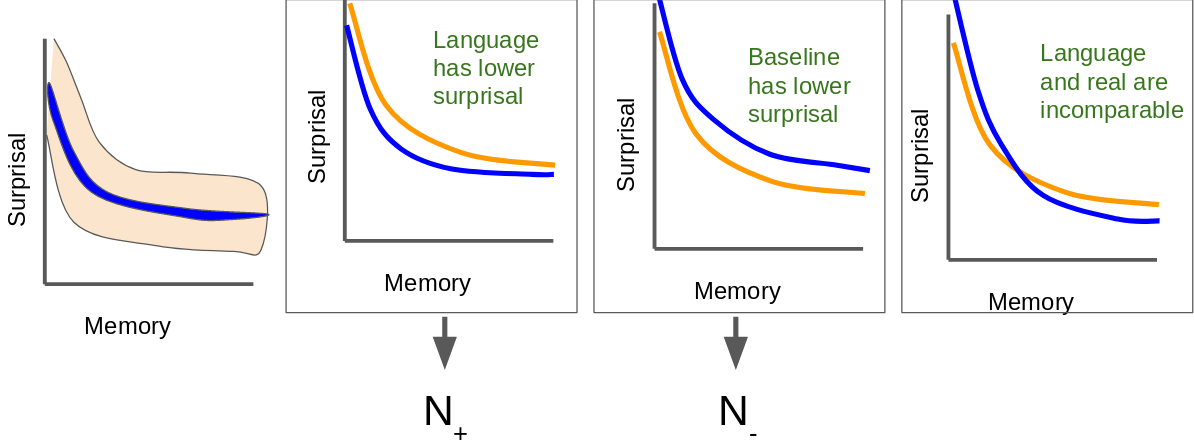
\includegraphics[width=0.45\textwidth]{figures/quantile-global.png}
\end{center}
	\caption{Illustration for the global quantile estimate. For each sample for the real language, we compare the memory-surprisal curve to all baselines.}\label{fig:quantile-global}
\end{figure}



For each sample $x$ from real orderings, we look at the proportions $N_+(x)$ of samples from the baseline languages that are more optimal than $x$ throughout the entire range where both curves are defined, and the proportion $N_-(x)$ of baseline samples that are consistently less optimal.

%We consider the null hypothesis that, on average, not more baseline languages are consistently less optimal than are consistently more optimal than the real orderings:
%\begin{equation}
%	\E_{x \sim P_1}[W_+(x)] \geq \E_{x \sim P_1}[W_-(x)]
%\end{equation}

We estimate the quotient
\begin{equation}\label{eq:g}
	G :=	\frac{\E_{x \sim P_1}[W_+(x)]}{\E_{x \sim P_1}[W_+(x) + W_-(x)]}
\end{equation}
where $P_1$ is the distribution over values obtained for real orderings.
We use a bootstrapped confidence interval for $\E[G]$ for quantifying the degree of optimization.
For bootstrapping, we separately resample samples from the real language and from the baseline grammars.

Unlike the other statistics, this one provides a global measure of the degree of optimization of the real language.
Due to the use of bootstrapping, the confidence intervals are not exact.


%- bootstrapping
%- subsampling
%- permutation test / rank test ??
%



\subsection{Number of Samples}
Training neural language models is computationally costly.
Therefore, we used a precision-based stopping criterion to adaptively choose a sample size for each language.
Precision-based stopping criteria offer a way to adaptively choose sample size without biasing results (CITE).

For each language, we first collected 10 data points for real orderings and 10 data points for baseline orderings.
We continued obtaining new data points until the CI for $G$ had width $\leq 0.15$, or there were 100 samples from $P_1$ and 300 samples from $P_2$.
Up to the end, we chose the next sample to be from $P_0$ with probability 2/3, and $P_1$ otherwise.\footnote{Due to a scripting error, a much higher number of samples was generated for Erzya.}

This procedure was parallelized on several machines.
In the case where the stopping criterion was reached for a language while several machines were still computing samples for this language, we did not discard those samples.
Consequently, more samples were collected than necessary to reach the stopping criterion; however, in a way that does not bias our results towards or against our hypothesis.

%Due to parallelization of this procedure, it often produced more samples than required, when the stopping criterion .
%We chose these thresholds based on preliminary simulations which had suggested that these widths were achievable at acceptable computational cost.
%For each language, we collected at least 5 data points for real orderings and at least 10 data points for baseline orderings.
%We continued obtaining new data points until the CI for $G$ had width $\leq 0.15$, or there were 100 samples from $P_1$ and 300 samples from $P_2$.
%Up to the end, we chose the next sample to be from $P_0$ with probability 2/3, and $P_1$ otherwise.




\subsection{Results}

The numbers of samples taken per language are provided in Table~\ref{tab:samples}.

%In Figure~\ref{tab:plain-results} (TODO), we show the estimated memory-surprisal tradeoff curves for all samples.

In Figure~\ref{tab:medians}, we show the medians for real and baseline languages.

Descriptively, the real language provides better tradeoffs than the median of the baselines across languages, with four exceptions (Latvian, North Sami, Polish, Slovak).

In Figure~\ref{tab:slice-hists-real}, we show the distribution of surprisals achieved at the maximal memory value for real and random languages.

In Figure~\ref{fig:hist-real}, we show surprisals at maximum memory, after z-transforming for each individual language and then aggregating.

In Table \ref{tab:median_diffs}, we show the differences in median surprisal, as a function of memory.


In Table~\ref{tab:boot-g}, we report the bootstrap estimates and confidence intervals for G~(\ref{eq:g}).
$\E[G]$ was not estimated to be significantly above $>5$ for four languages: Latvian, North Sami, Polish, and Slovak.


In Table~\ref{tab:quantiles}, we show the quantiles.





\subsection{Discussion}

We have found that 48 out of 52 languages provide better memory-surprisal tradeoffs than random baselines with consistent but counterfactual word order rules.

Four languages provide exceptions; these are Latvian (Baltic), North Sami (Uralic), Polish and Slovak (both Slavic).
All four languages have strong word order freedom (CITE).
Freedom of word order plausibly makes sentences less predictable, as the same syntactic structure can receive different surface realizations.
We thus hypothesized that freedom of word order impacts the memory-surprisal tradeoff, and that languages with more strongly fixed word order should display more optimal memory-surprisal tradeoffs.
%We hypothesized that freedom of word order freedom may be responsible for the difference between these languages and the other languages.

To test this hypothesis, we examined the correlation between word order freedom and the surprisal difference between real and baseline orderings.
To quantify word order freedom, we used a corpus-based estimate, the \emph{branching direction entropy}~\citep{futrell-quantifying-2015}.
This is the entropy of the ordering (head-first or dependent-first) of dependencies conditioned on the dependency label and the part-of-speech label of head and dependent.
%\cite{futrell-quantifying-2015} showed that this me
These two quantities are plotted in Figure~\ref{fig:hist-real}.
We found that branching direction entropy was strongly correlated with the surprisal difference between real and baseline orderings (Spearman correlations -0.58, $p = 7.414e-6$).



\begin{figure}
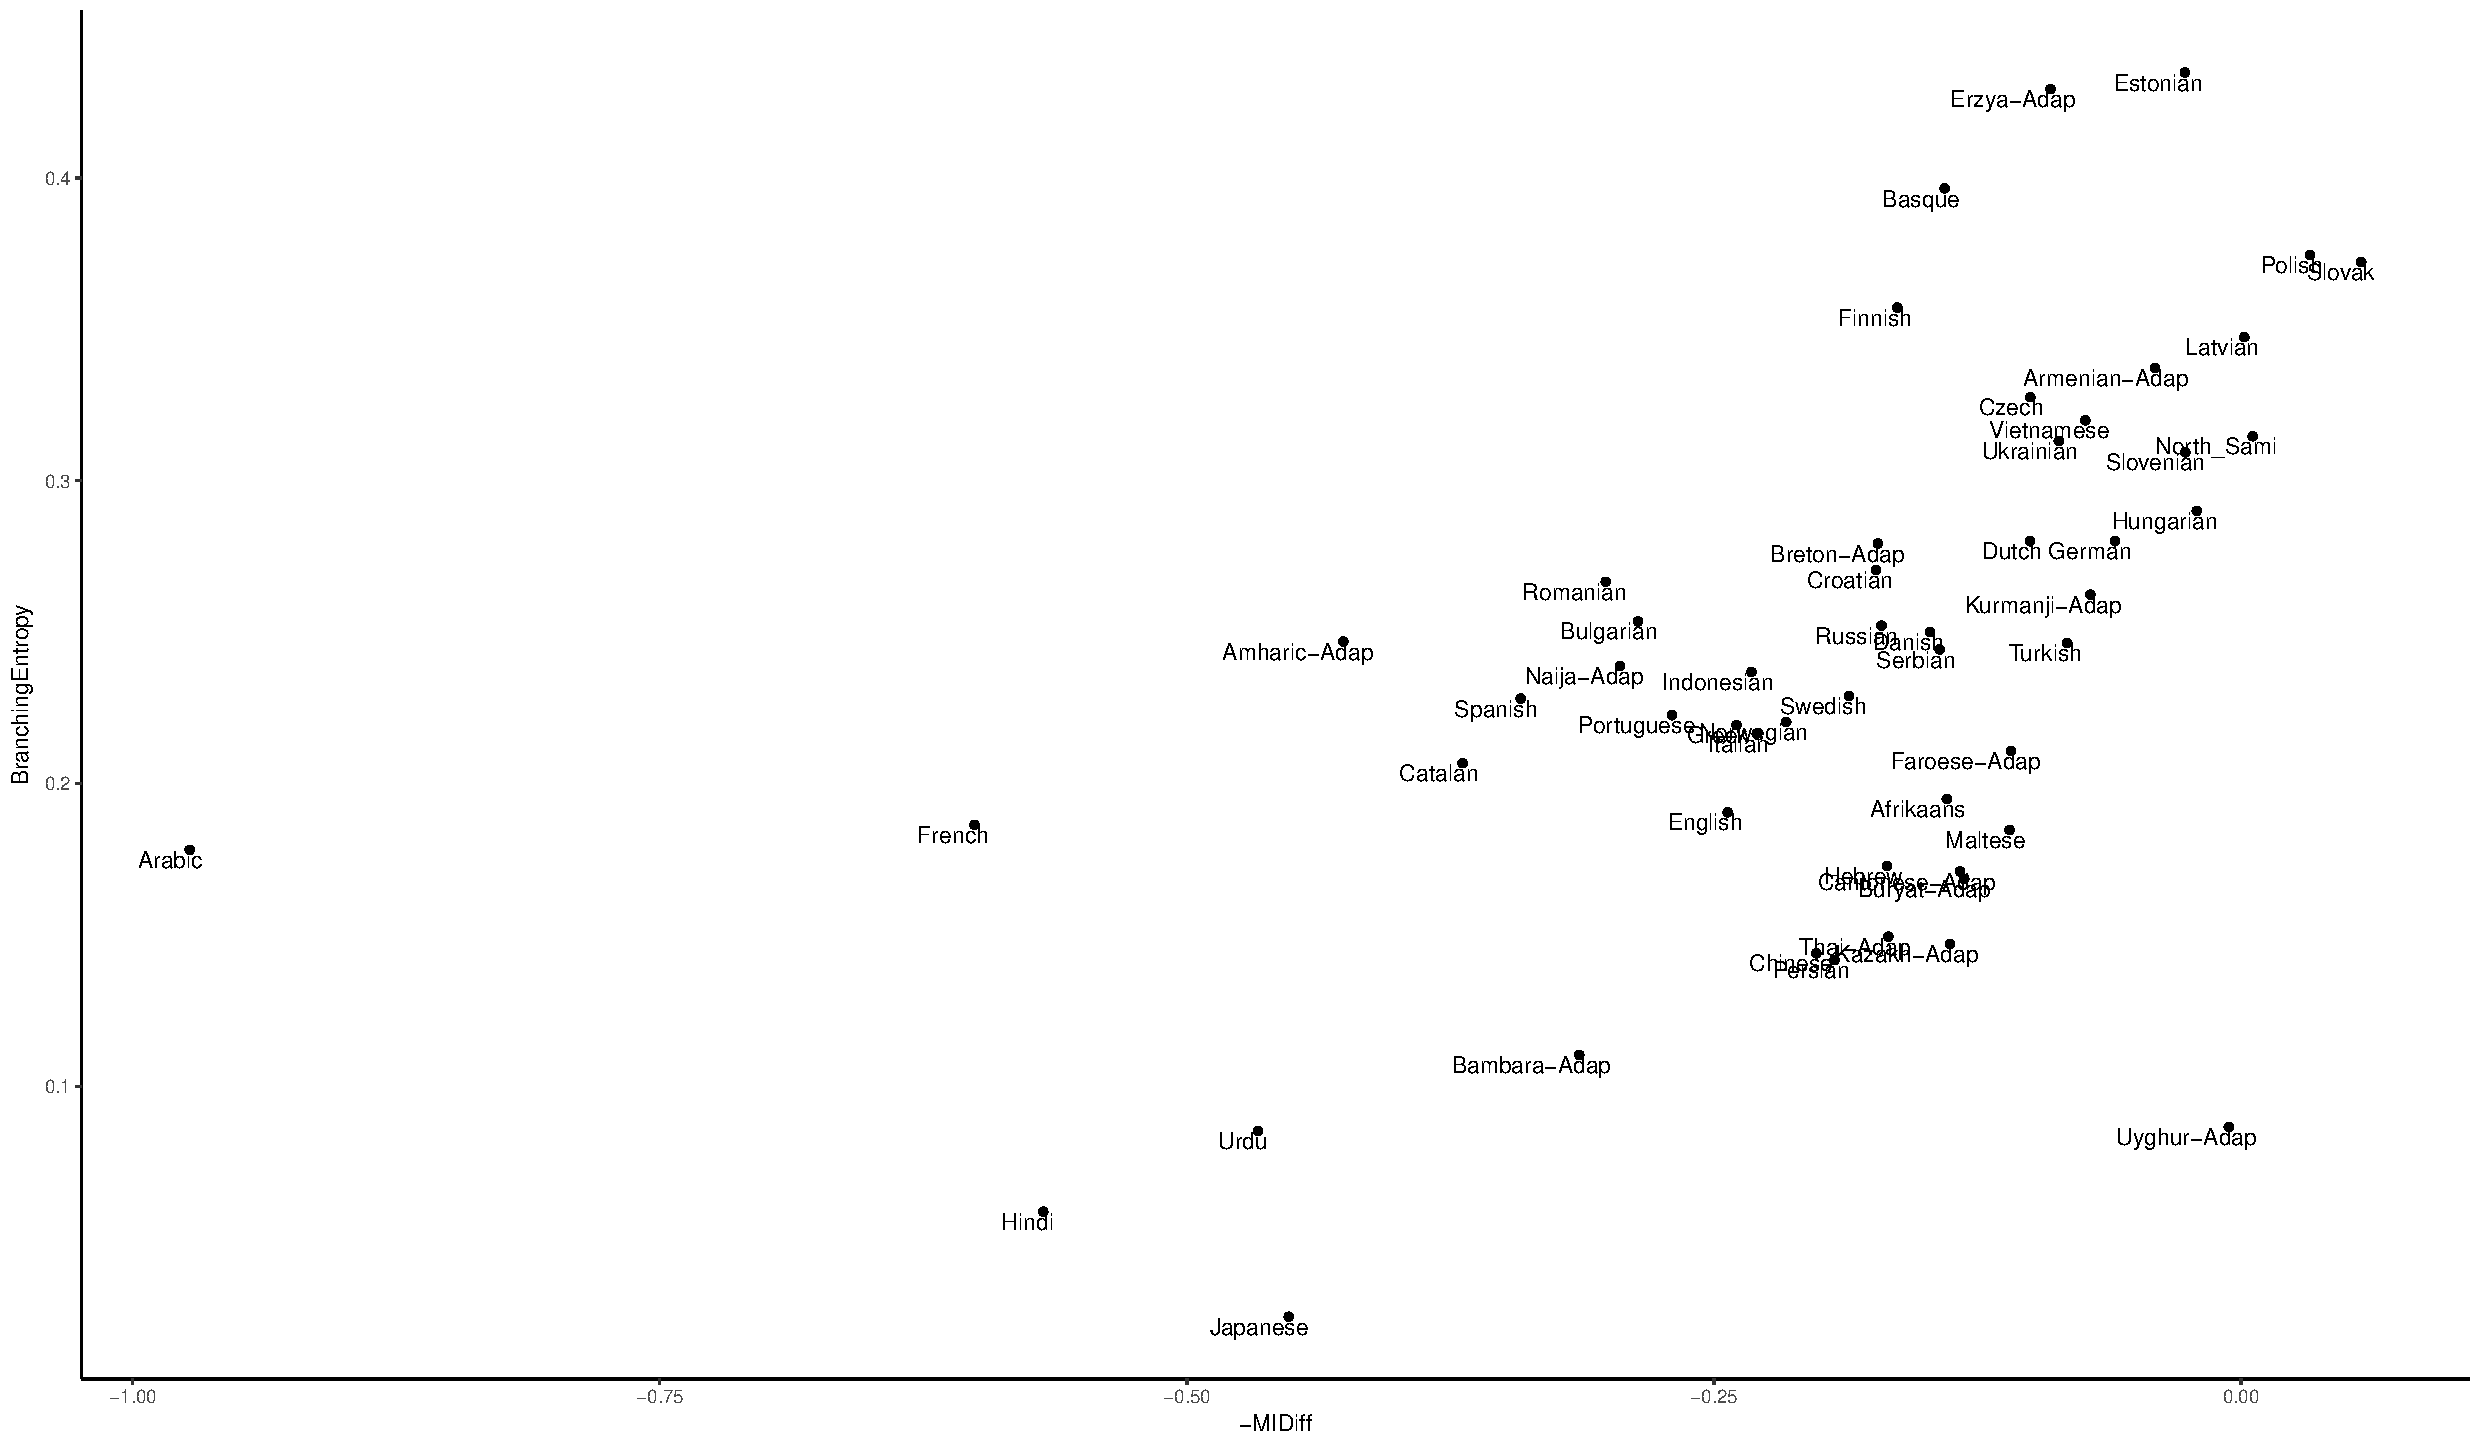
\includegraphics[width=0.95\textwidth]{../code/analyze_neural/figures/surprisal-branching-entropy-REAL.pdf}
	\caption{Surprisal Difference vs Branching Direction Entropy.}\label{fig:hist-real}
\end{figure}






\section{Experiment 3: Fixed Word Orders}

We test this hypothesis by comparing baseline languages to \emph{fixed-order} versions of the real languages.
This enables us to tease apart the impact of the languages' word order rules from the impact of word order freedom.


\begin{figure}
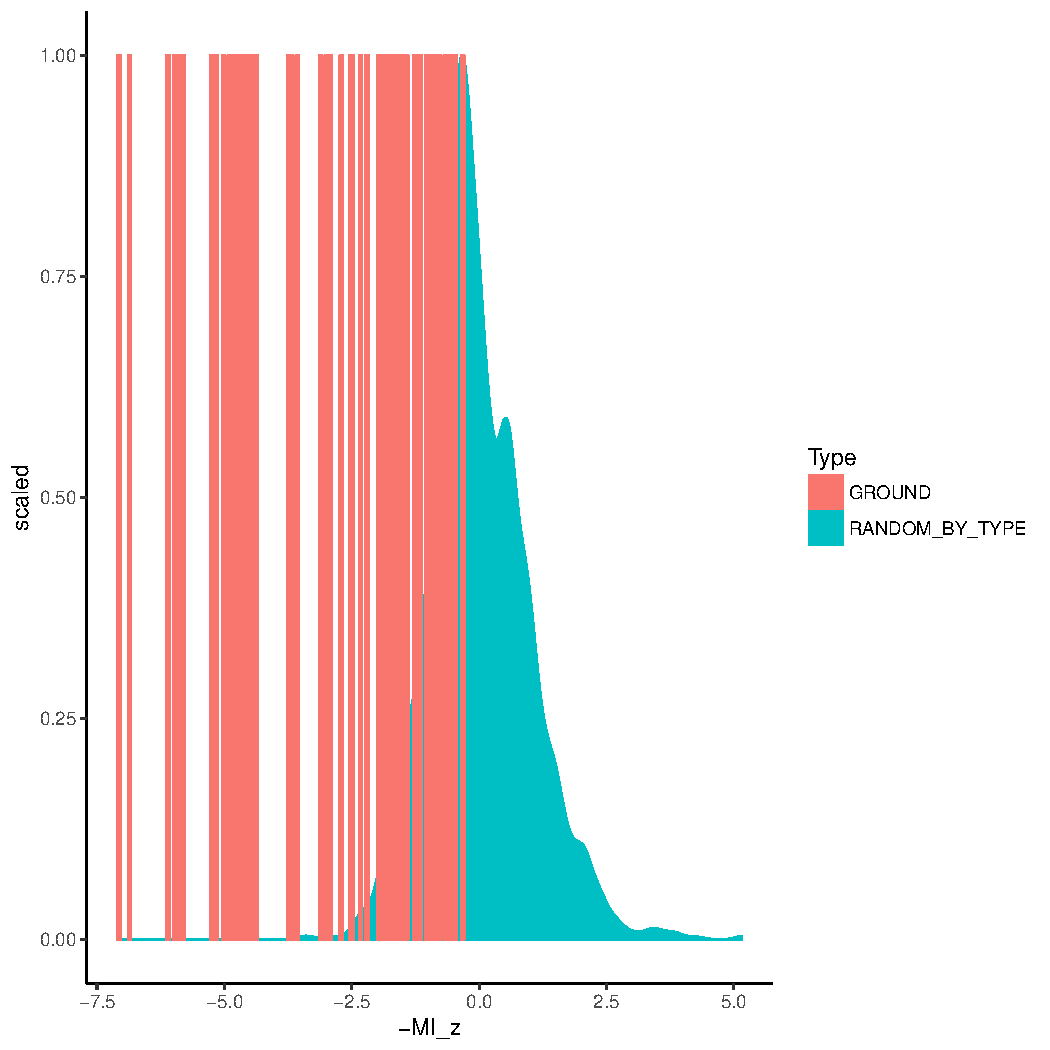
\includegraphics[width=0.5\textwidth]{../code/analyze_neural/figures/full-GROUND-listener-surprisal-memory-HIST_z_byMem_onlyWordForms_boundedVocab.pdf}
	\caption{Histogram}\label{fig:hist-real}
\end{figure}



\paragraph{Fitting Ordering Grammars to Actual Orders}
We create ordering grammars that are fit to the actual orderings of each language.
These grammars faithfully represent the ordering rules if the actual language, to the extent that is possible in the formalism of ordering grammars.

We construct these grammars by constructing \emph{probabilistic ordering grammars}, and setting the parameters to maximize the \emph{likelihood} of the actually observed orderings.
We parameterized probabilistic ordering grammars as follows.
For each relation type $\tau$, we introduce a \emph{direction parameter} $a_\tau \in [0,1]$ and a \emph{distance parameter} $b_\tau \in \mathbb{R}$.
Each dependent is ordered on the left of its head with probability $a_\tau$ and to the right with probability $1-a_\tau$. 
Then for each set of co-dependents $\{s_1, \dots , s_n\}$ placed on one side of a head, their order outward from the head is determined by iteratively sampling from the distribution $\operatorname{softmax}(b_{\tau_1}, \dots, b_{\tau_n})$ (\cite{goodfellow2016deep}, p. 184) without replacement. 

Given a dependency tree, a probabilistic ordering grammar assigns a probability distribution over the possible projective linearizations of that tree.
We use gradient descent to find parameters $a_\tau, b_\tau$ so as to maximize the overall likelihood of the orders in the actual corpus.


We convert probabilistic ordering grammars into ordinary ordering grammars by the following method.
Let $A_-$ be those relations $\tau$ where $a_\tau > 0.5$, similarly for $A_+$ those here $a_\tau \geq 0.5$.
Then we order all relations in $A_-$ by $b_\tau$ in \emph{decreasing} order, and those in $A_+$ by $b_\tau$ in \emph{increasing} order.

Then ordering a tree following the converted version is equivalent to greedily choosing the highest-probability linearization for the dependents of each head in a tree.


We choose this method since maximum-likelihood grammars can be constructed with simple gradient descent.
Another option would be to use some kind of discrete optimization method to approximate the original orders without a probabilistic method.
However, discrete optimization is computationally challenging.

\paragraph{Results}


